\documentclass[11pt]{article}
\usepackage{listings}
\usepackage{tikz}
\usepackage{enumerate}
\usetikzlibrary{arrows,automata,shapes}

\newtheorem{defn}{Definition}
\newtheorem{crit}{Criterion}

\newcommand{\handout}[5]{
  \noindent
  \begin{center}
  \framebox{
    \vbox{
      \hbox to 5.78in { {\bf Software Testing, Quality Assurance and Maintenance } \hfill #2 }
      \vspace{4mm}
      \hbox to 5.78in { {\Large \hfill #5  \hfill} }
      \vspace{2mm}
      \hbox to 5.78in { {\em #3 \hfill #4} }
    }
  }
  \end{center}
  \vspace*{4mm}
}

\newcommand{\lecture}[4]{\handout{#1}{#2}{#3}{#4}{Lecture #1}}
% 1-inch margins, from fullpage.sty by H.Partl, Version 2, Dec. 15, 1988.
\topmargin 0pt
\advance \topmargin by -\headheight
\advance \topmargin by -\headsep
\textheight 8.9in
\oddsidemargin 0pt
\evensidemargin \oddsidemargin
\marginparwidth 0.5in
\textwidth 6.5in

\parindent 0in
\parskip 1.5ex
%\renewcommand{\baselinestretch}{1.25}

% http://gurmeet.net/2008/09/20/latex-tips-n-tricks-for-conference-papers/
\newcommand{\squishlist}{
 \begin{list}{$\bullet$}
  { \setlength{\itemsep}{0pt}
     \setlength{\parsep}{3pt}
     \setlength{\topsep}{3pt}
     \setlength{\partopsep}{0pt}
     \setlength{\leftmargin}{1.5em}
     \setlength{\labelwidth}{1em}
     \setlength{\labelsep}{0.5em} } }
\newcommand{\squishlisttwo}{
 \begin{list}{$\bullet$}
  { \setlength{\itemsep}{0pt}
     \setlength{\parsep}{0pt}
    \setlength{\topsep}{0pt}
    \setlength{\partopsep}{0pt}
    \setlength{\leftmargin}{2em}
    \setlength{\labelwidth}{1.5em}
    \setlength{\labelsep}{0.5em} } }
\newcommand{\squishend}{
  \end{list}  }

\begin{document}

\lecture{8 --- January 21, 2015}{Winter 2015}{Patrick Lam}{version 1}

Another coverage criterion that I've mentioned, but is not in the notes:
\begin{crit}
{\bf Specified Path Coverage}. (SPC) \emph{TR} contains a specified set $S$ of
paths.
\end{crit}

Specified path coverage might be useful for encoding a set of usage scenarios.

\paragraph{Prime Path Coverage versus Complete Path Coverage.}

\begin{center}
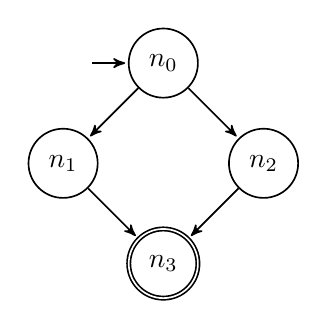
\begin{tikzpicture}[->,>=stealth',shorten >=1pt,auto,node distance=1.8cm,
                    semithick,initial text=]

  \node[initial,state]   (0)                    {$n_0$};
  \node[state]           (1) [below left of=0]  {$n_1$};
  \node[state]           (2) [below right of=0] {$n_2$};
  \node[accepting,state] (3) [below right of=1] {$n_3$};
  
  \path (0) edge              node {} (1)
        (0) edge              node {} (2)
        (2) edge              node {} (3)
        (1) edge              node {} (3);
\end{tikzpicture}
\end{center}

\begin{itemize}
\item {\sf Prime paths: }
\item $\mbox{path}(t_1) = $ 
\item $\mbox{path}(t_2) = $ 
\item $T_1 = \{ t_1, t_2 \}$ satisfies both PPC and CPC.
\end{itemize}

\begin{center}
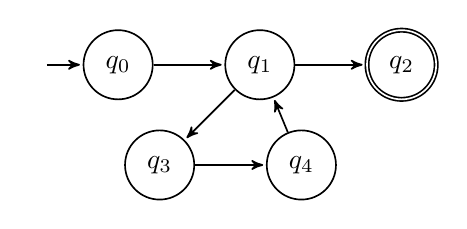
\begin{tikzpicture}[->,>=stealth',shorten >=1pt,auto,node distance=1.8cm,
                    semithick,initial text=]

  \node[initial,state]   (1)              {$q_0$};
  \node[state] (4) [right of=1] {$q_1$};
  \node[state] (5) [below left of=4] {$q_3$};
  \node[state] (6) [right of=5] {$q_4$};
  \node[accepting,state] (7) [right of=4] {$q_2$};
  
  \path (1) edge              node {} (4)
        (4) edge              node {} (7)
        (4) edge              node {} (5)
        (5) edge              node {} (6)
        (6) edge              node {} (4);
\end{tikzpicture}
\end{center}

\begin{itemize}
\item {\sf Prime paths: }
\item $\mbox{path}(t_3) = $ 
\item $\mbox{path}(t_4) = $ 
\item $T_1 = \{ t_3, t_4 \}$ satisfies both PPC but not CPC.
\end{itemize}

Now, we'll see another graph theory-inspired coverage criterion. First, some definitions:
\begin{defn}
  A graph $G$ is \emph{connected} if every node in $G$ is reachable from the
  set of initial nodes $N_0$.
\end{defn}
\begin{defn}
  An edge $e$ is a \emph{bridge} for a graph $G$ if $G$ is connected,
  but removing $e$ from $G$ results in a disconnected graph.
\end{defn}
(This is similar to an articulation point in a graph, except that
articulation points are nodes, not edges.)

\begin{crit}
  {\bf Bridge Coverage.} (BC) \emph{TR} contains all bridges.
\end{crit}
Assume that a graph contains at least two nodes, and all nodes
in a graph are reachable from the initial nodes. Does bridge
coverage subsume node coverage? Justify your answer, providing
a counterexample if appropriate.

\paragraph{Specifying versus meeting test requirements.}
Consider this graph.

\begin{center}
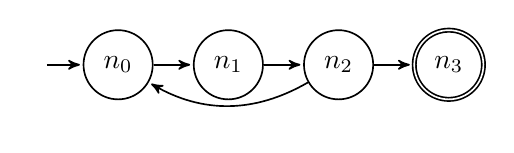
\begin{tikzpicture}[->,>=stealth',shorten >=1pt,auto,node distance=1.4cm,
                    semithick,initial text=]

  \node[initial,state]   (1)              {$n_0$};
  \node[state]           (2) [right of=1] {$n_1$};
  \node[state]           (3) [right of=2] {$n_2$};
  \node[accepting,state] (4) [right of=3] {$n_3$};
  
  \path (1) edge              node {} (2)
        (2) edge              node {} (3)
        (3) edge [bend left]  node {} (1)
        (3) edge              node {} (4);
\end{tikzpicture}
\end{center}

{\sf The following simple (and loop-free) path is, in fact, prime: }
\[ p = %[n_0, n_1, n_2, n_3]
\]
PPC includes this path as a test requirement. The \emph{test path}
\[ %[n_0, n_1, n_2, n_0, n_1, n_2, n_3]
\] meets the test requirement induced by $p$ even though it is not prime.
Note that a test path may satisfy the prime path test requirement even though
it is not prime.

\paragraph{Graph Coverage Exercise.} Consider the graph defined
by the following sets.
\squishlist
\item $N = \{1, 2, 3, 4, 5, 6, 7\}$
\item $N_0 = \{ 1 \}$
\item $N_f = \{ 7 \}$
\item $E = \{ [1, 2], [1, 7], [2, 3], [2,4], [3, 2], [4,5], [4, 6], [5, 6], [6, 1] \}$
  \squishend
  Also consider the following test paths:
  \squishlist
\item $t_0 = [1, 2, 4, 5, 6, 1, 7]$
\item $t_1 = [1, 2, 3, 2, 4, 6, 1, 7]$
  \squishend

Answer the following questions.
\begin{enumerate}[(a)]
\item Draw the graph.
\item List the test requirements for EPC. [hint: 12 requirements of length 2]
\item Does the given set of test paths satisfy EPC? If not, identify what is missing.
\item Consider the simple path $[3,2,4,5,6]$ and test path $[1,2,3,2,4,6,1,2,4,5,6,1,7]$. Is the simple path a subpath of the test path?
\item List the test requirements for NC, EC, and PPC on this graph.
\item List a test path that achieves NC but not EC on the graph.
\item List a test path that achieves EC but not PPC on the graph.
\end{enumerate}
(Note: We've talked about test sets meeting criteria in the past.  For
(f) and (g), we are simply talking about a test set with one test case
that induces the given test paths.)

\end{document}
